\documentclass[tikz,border=10pt]{standalone}
\begin{document}
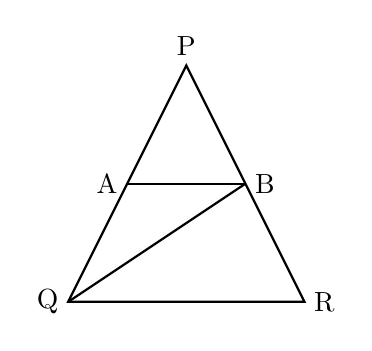
\begin{tikzpicture}[scale=1]

    % Define coordinates
    % P is the top vertex
    \coordinate (P) at (0, 3);
    % Q and R are the bottom vertices
    \coordinate (Q) at (-1.5, 0);
    \coordinate (R) at (1.5, 0);

    % A is on the line segment PQ
    \coordinate (A) at (-0.75, 1.5);
    % B is on the line segment PR
    \coordinate (B) at (0.75, 1.5);

    % Draw the main triangle PQR
    \draw[thick] (P) -- (Q) -- (R) -- cycle;

    % Draw the horizontal line segment AB
    \draw[thick] (A) -- (B);

    % Draw the diagonal line segment QB
    \draw[thick] (Q) -- (B);

    % Add labels for the points
    % Adjusting positions to match the image
    \node[above] at (P) {P};
    \node[left] at (Q) {Q};
    \node[right] at (R) {R};
    \node[left] at (A) {A};
    \node[right] at (B) {B};

\end{tikzpicture}
\end{document}
